\chapter{Algorithme 3}

\section{Présentation}

Le troisième algorithme applique la technique du NEE en chaque point intermédiaire. Ainsi, chaque point $p_k$ sera connecté au récepteur où sa contribution sera prise en compte.

\section{Découpe du rayon}

Ici, il faut procéder comme pur l'algorithme 3, mais les foyers de l'ellipse seront les point $x_i$ et $M_{rx}$ puisque nous voulons connecter chaque point intermédiaire $p$ au récepteur afin d'appliquer le NEE (et non plus à l'émetteur).

\begin{figure}[h!]
\centering
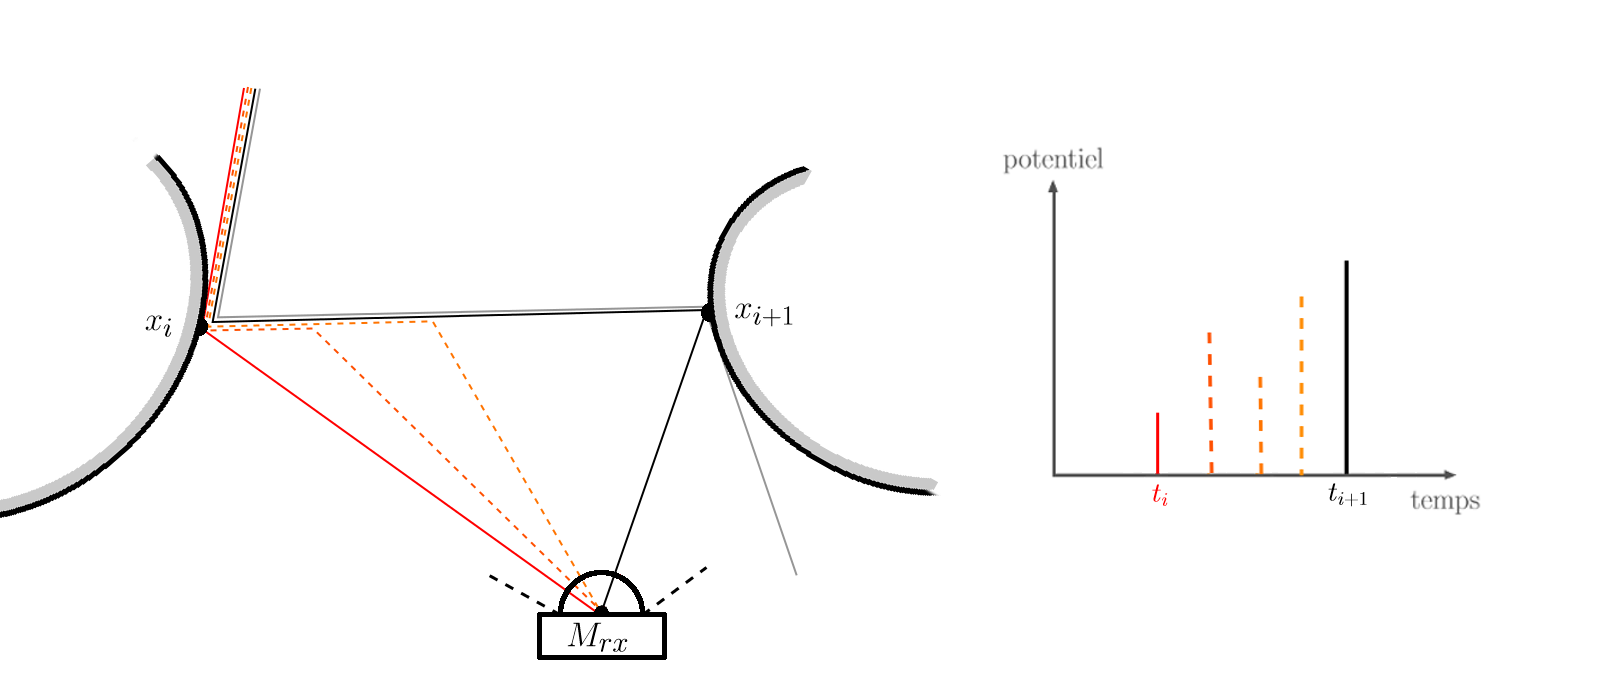
\includegraphics[width=180mm]{find_ray_decomposition_Rx.png}
\caption{Décomposition du rayon et réponse impulsive correspondante}
\end{figure}

\begin{figure}[h!]
\centering
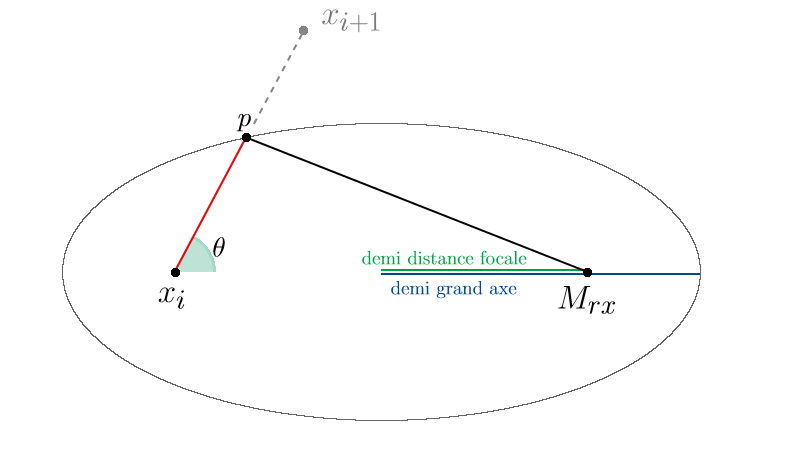
\includegraphics[width=180mm]{ellipseRx.png}
\caption{Utilisation de l'ellipse pour trouver la distance $x_i p$}
\end{figure}

\section{Algorithme}

Je rajoute, une méthode \textbf{outScatteringAlongARay} qui gère la connexion au récepteur $M_{rx}$ pour chaque point intermédiaire (point de milieu), en simulant la réception par le récepteur, et en complétant la réponse impulsionnelle.

\section{Résultats}

Suite à un problème avec Scilab, je n'ai pas pu réaliser des graphes comme à l'algo 1, c'est-à-dire un graphe par profondeur.

\subsection{Coefficient de dispersion}

Dans un premier temps, nous regardons l'impact du coefficient de dispersion sur les contributions lumineuses. Ainsi :
\begin{itemize}
    \item le coefficient d'atténuation $\sigma_a$ vaut 0 ;
    \item le paramètre g vaut 0 : le milieu est complètement isotropique.
    \item la densité du milieu est de 1 ;
    \item 3 réflexions.
\end{itemize}
\vspace{1em}\par

En lançant $10^7$ rayons, nous obtenons le résultat de la figure \ref{fig:resultats_algo3_dispersion}.\newline

\begin{figure}[h!]
\centering
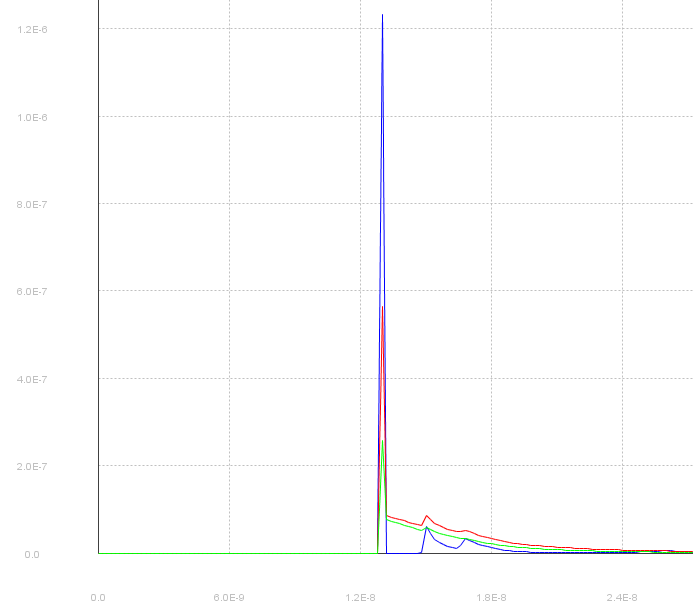
\includegraphics[width=150mm]{resultats/algo3/algo_3_resultats.PNG}
\caption{
bleu : $\sigma_s = 0.0$ \qquad
rouge : $\sigma_s = 0.2$ \qquad
vert : $\sigma_s = 0.4$}
\label{fig:resultats_algo3_dispersion}
\end{figure}

On remarque que l'out-scattering produit dans un premier temps un effet d'amplification de la lumière. Le récepteur reçoit en permanence des rayons qui viennent contribuer, même faiblement. Cela dit, au bout d'un moment le coefficient d'extinction devient trop fort et la lumière est tellement atténuée que les contributions de l'out-scattering ne sont plus suffisantes pour avoir un gain de lumière.

\subsection{Paramètre g}

Rappelons que le paramètre $g$ d'un milieu participant indique si celui-ci est isotropic ($g = 0$), induit une majorité de backward-scattering ($-1 < g < 0$) ou une majorité de forward-scattering ($0 < g < 1$) (cf section \ref{explication_parametre_g}).\par
Pour les résultats suivants, je n'ai fait varier que le paramètre g et les autres valeurs étaient :
\begin{itemize}
    \item le coefficient d'atténuation $\sigma_a$ vaut 0 ;
    \item le coefficient de dispersion $\sigma_s$ vaut 0.2 ;
    \item la densité du milieu est de 1 ;
    \item 3 réflexions.
\end{itemize}

\begin{figure}[h!]
\centering
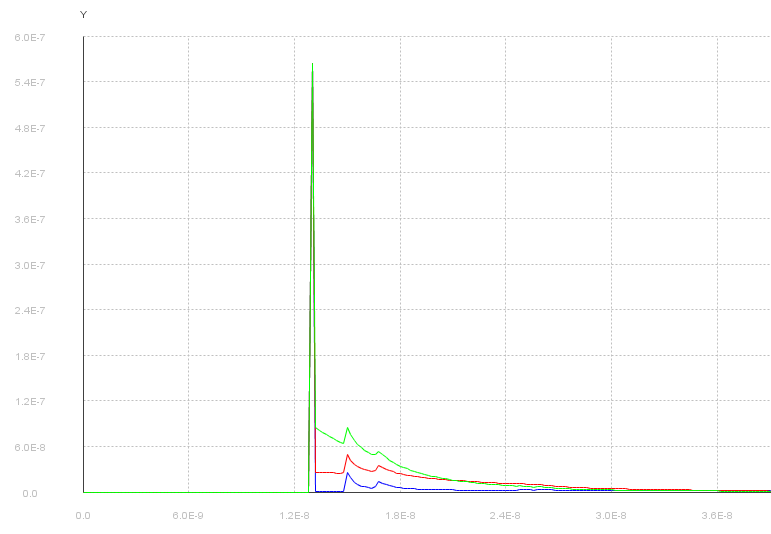
\includegraphics[width=150mm]{resultats/algo3/backward_scattering.PNG}
\caption{backward-scattering : \qquad
vert : $g = 0$ \qquad
rouge : $g = -0.5$ \qquad
bleu : $g = -0.9$}
\end{figure}

\begin{figure}[h!]
\centering
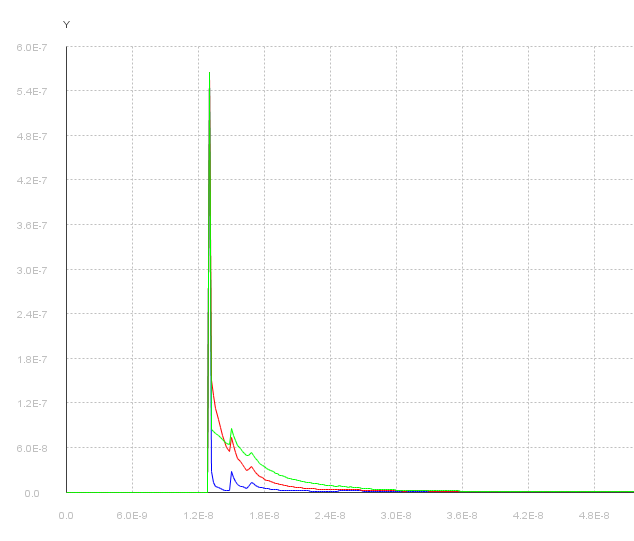
\includegraphics[width=150mm]{resultats/algo3/forward_scattering.PNG}
\caption{forward-scattering : \qquad
vert : $g = 0$ \qquad
rouge : $g = 0.5$ \qquad
bleu : $g = 0.9$}
\end{figure}